\documentclass{article}
\usepackage{tikz}
\usetikzlibrary{arrows.meta}

\begin{document}

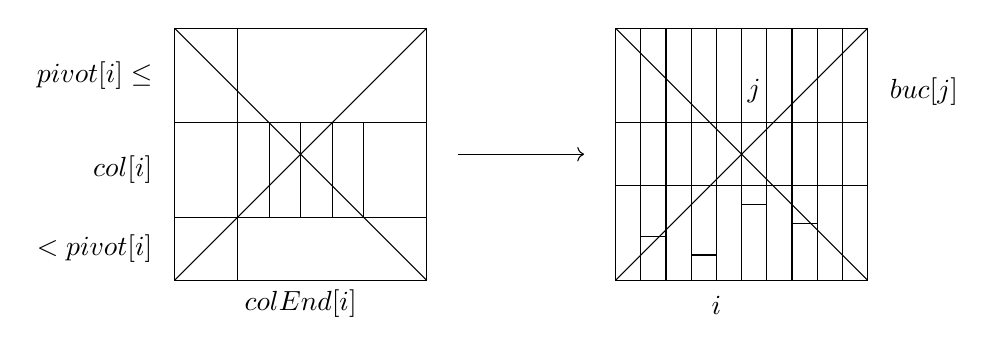
\begin{tikzpicture}[scale=0.8]
% Left matrix
\draw (0,0) rectangle (4,4);

% Horizontal divisions in left matrix
\draw (0,1) -- (4,1);
\draw (0,2.5) -- (4,2.5);

% Vertical divisions in left matrix
\draw (1,0) -- (1,4);
\draw (1.5,1) -- (1.5,2.5);
\draw (2,1) -- (2,2.5);
\draw (2.5,1) -- (2.5,2.5);
\draw (3,1) -- (3,2.5);

% Right matrix
\draw (7,0) rectangle (11,4);

% Vertical divisions in right matrix
\draw (7.4,0) -- (7.4,4);
\draw (7.8,0) -- (7.8,4);
\draw (8.2,0) -- (8.2,4);
\draw (8.6,0) -- (8.6,4);
\draw (9,0) -- (9,4);
\draw (9.4,0) -- (9.4,4);
\draw (9.8,0) -- (9.8,4);
\draw (10.2,0) -- (10.2,4);
\draw (10.6,0) -- (10.6,4);

% Horizontal divisions in right matrix
\draw (7,1.5) -- (11,1.5);
\draw (7,2.5) -- (11,2.5);

% Irregular heights in right matrix
\draw (7.4,0) -- (7.4,0.7) -- (7.8,0.7) -- (7.8,0);
\draw (8.2,0) -- (8.2,0.4) -- (8.6,0.4) -- (8.6,0);
\draw (9,0) -- (9,1.2) -- (9.4,1.2) -- (9.4,0);
\draw (9.8,0) -- (9.8,0.9) -- (10.2,0.9) -- (10.2,0);

% Arrow between matrices
\draw[->] (4.5,2) -- (6.5,2);

% Diagonal lines in left matrix
\draw (0,0) -- (4,4);
\draw (0,4) -- (4,0);

% Diagonal lines in right matrix
\draw (7,0) -- (11,4);
\draw (7,4) -- (11,0);

% Labels for left matrix
\node[left] at (-0.2,3.25) {$pivot[i] \leq$};
\node[left] at (-0.2,1.75) {$col[i]$};
\node[left] at (-0.2,0.5) {$< pivot[i]$};
\node[below] at (2,0) {$colEnd[i]$};

% Labels for right matrix
\node at (9.2,3) {$j$};
\node[right] at (11.2,3) {$buc[j]$};
\node[below] at (8.6,-0.1) {$i$};

\end{tikzpicture}

\end{document}